\documentclass[journal]{vgtc}
\let\ifpdf\relax
\usepackage{hs-vis_ss10}


%% Please note that the use of figures other than the optional teaser
%% is not permitted on the first page of the journal version.  Figures
%% should begin on the second page and be in CMYK or Grey scale
%% format, otherwise, colour shifting may occur during the printing
%% process.  Papers submitted with figures other than the optional
%% teaser on the first page will be refused.

%% These three lines bring in essential packages: ``mathptmx'' for
%% Type 1 typefaces, ``graphicx'' for inclusion of EPS figures. and
%% ``times'' for proper handling of the times font family.

\usepackage{mathptmx}
\usepackage{amsmath}
\usepackage{amssymb}
\usepackage{graphicx}
\usepackage{times}


%% allow for this line if you want the electronic option to work
%% properly
\vgtcinsertpkg


%% author name
\author{Steffen Fuchs}

%% paper title
\title{Objektsegmentierung im Video: Ein hierarchischer, variationaler Ansatz, um Punkttrajektorien auf dichte Regionen zu erweitern}

%% short title for header
\shorttitle{Objektsegmentierung im Video}


%% Abstract section.
\abstract{%
  Punkttrajektorien zeichneten sich in der Vergangenheit als leistungsstarkes Hilfsmittel ab, um unbeaufsichtigt qualitativ hochwertige
  Segmentierungen auf Videosequenzen durchzuführen. Sie können zwar die Langzeit-Bewegungsunterschiede zu ihrem Vorteil nutzen,
  liefern auf Grund ihres Rechenaufwandes und der Schwerigkeiten in homogenen Regionen in der Regel aber nur spärliche Informationsdichte.
  Die Authoren P. Ochs und T.Brox stellen mit ihrer Arbeit eine variationale Methode vor, um aus den Gruppierungen dieser grob verteilten
  Trajektorien eine dichte Segmentierung zu gewinnen.  Die Information wird dabei durch einen hierarchischen, nicht-linearen Diffusionsprozesses
  propagiert, welcher zwar im kontinuierlichen Bereich arbeitet, jedoch Superpixel mit berücksichtigt.
  Es wird gezeigt, dass dieser Prozess nicht nur die Informationsdichte von 3\% auf 100\% erhöht, sondern auch die durchschnittliche Genauigkeit der Labels
  verbessert.
} % end of abstract

%\begin{figure}[tb]\centering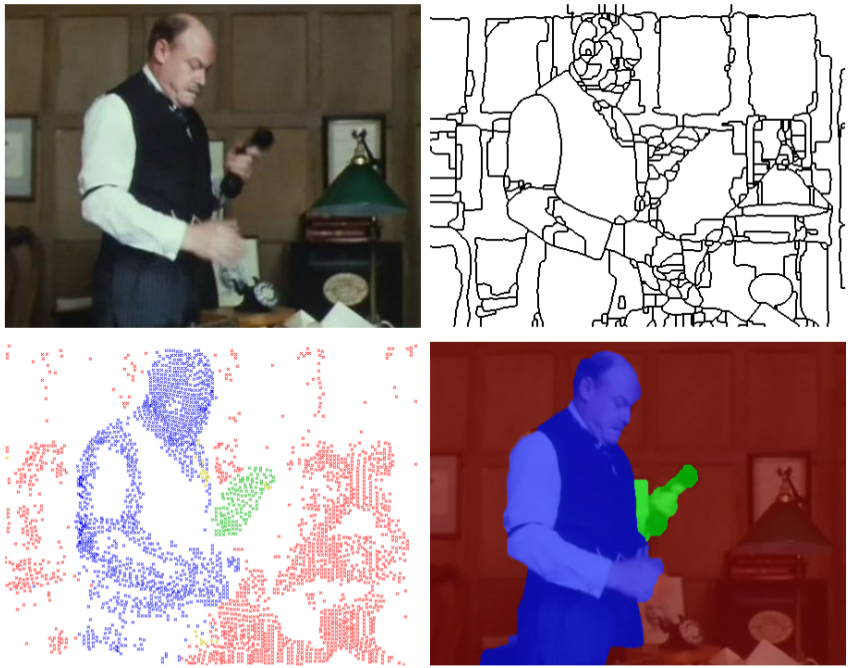
\includegraphics[width=3.5in]{images/teaser.png}
%  \caption{}\label{fig:teaser}
%\end{figure}


%% Uncomment below to include a (optional) teaser figure.
\teaser{ \centering
  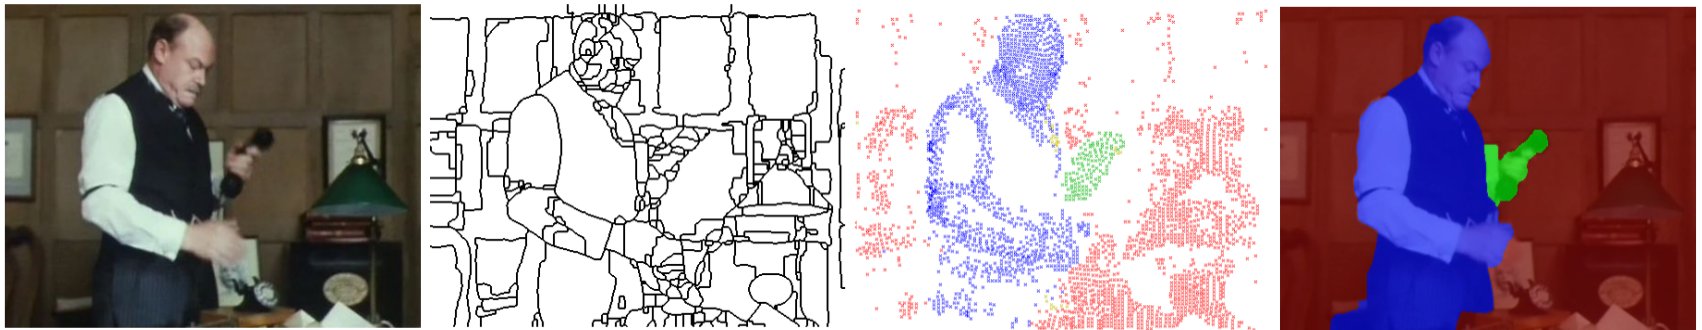
\includegraphics[width=16cm]{images/teaser2.png}
  \caption{von links nach rechts: original Bild, statische Segmentierung, Segmentierung auf Punkttrajektorien, hier vorgestelltes Verfahren.
   Klassische, statische Bildsegmentierungsverfahren wie \cite{001} führen häufig zu Übersegmentierungen, während
   Objektsegmentierungen, die ausschließlich Punkttrajektorien verwenden \cite{007}, nur unvollständige Labelinformationen liefern.
   Die Authoren P. Ochs und T. Brox stellen ein hierarchisches, variationales Model vor, das Labels vorzugsweise in homogene Bereiche propagiert.
   Sie versuche somit, die Vorzüge beider Verfahren zu vereinen. Dadurch erhält man eine dichte Segmentierung,
   die darüberhinaus auch eine höhere Genauigkeit als die ursprünglichen Labels aufweist}
 \label{fig:teaser}
}


%%%%%%%%%%%%%%%%%%%%%%%%%%%%%%%%%%%%%%%%%%%%%%%%%%%%%%%%%%%%%%%%
%%%%%%%%%%%%%%%%%%%%%% START OF THE PAPER %%%%%%%%%%%%%%%%%%%%%%
%%%%%%%%%%%%%%%%%%%%%%%%%%%%%%%%%%%%%%%%%%%%%%%%%%%%%%%%%%%%%%%%%

\begin{document}

%% The ``\maketitle'' command must be the first command after the
%% ``\begin{document}'' command. It prepares and prints the title
%%   block.

%%   the only exception to this rule is the \firstsection command
\firstsection{Einleitung}
\maketitle
Aktuelle Lernansätze für visuelle Erkennung hängen sehr von der manuellen Markierung und Segmentierung von Objeckten ab.
Betrachtet man das bis heute beste visuelle Erkennungssystem - das menschliche Gehirn - wird klar,
dass solche manuellen Hilfestellungen nicht notwendig sind. Säuglinge erlernen die visuellen Formen und
Eigenschaften von Objekten auch ohne dass ihnen ihre Eltern Bounding Boxes darum legen oder eine Segmentierung zur Verfügung stellen.
Es gibt überzeugende Beweise darüber, dass Säuglinge dies Art von Objektsegmentierung durch Bewegungseinsatzen dürchführen \cite{}.
und man könnte letztendlich argumentieren, dass das rechnergestützte visuelle Systeme sich immer weiter dem menschlichen Sehvermögen annähren sollten.
\\
Die Bewegungsanalyse von Punkttrajektorien ist ein angemessens und robustes Werkzeug, um in Videosequenzen die Regionen von Objekten ohne
menschliches Zutun automatisch bestimmen und extrahieren zu können, wie in \cite{} erst kürzlich gezeigt.
Diese Ansätze verlangen jedoch danach, dass für die Bewegungsschätzung immer auch genügend Strukturen in den Bildern vorhanden sind,
zu denen Übereinstimmungen gefunden werden können.
In homogenen Gebieten gibt es diese Strukturen aber nicht, was dazu führt, dass die resultierenden Punkttrajektorien nur spärlich vorhanden sind.
In der Arbeit von \cite{} werden die Punkttrajektorien zwar aus dem dichten, optischen Flussfeld berechnet und resultierenden Trajektorien würden
ebenfalls für das gesamte Bild zur Verfügung stehen, jedoch sind diese in homogene Regionen weniger zuverlässig und können das Clustering behindern.
Zudem verlangen die eingeschränkte Verfügbarkeit von Rechenkraft nach der Reduzierung der Trajektorien, die analysiert werden sollen.
Das Clustern von dichten Punkttrajektorien würde viel zu lange dauern.
\\
Die Authoren stellten in ihrem Artikel eine Methode basierend auf der Variationsrechnung vor,
die aus wenigen Clustern von Punkttrajektorien eine dichte Segmentierung erstellt\ref{fig:01}.
Auf dem ersten Blick mag dies nach einem simplen Interpolationsproblem aussehen, da unser Verstand ganz einfach die Lücken zwischen den Punkten füllen kann.
Bei genaurer Betrachtung werden jedoch einige Schwierigkeiten deutlich.
So werden zum Beispiel einige der kritischen Bereich überhaupt nicht von den Trajektorien abgedeckt,
ganz besonders sind davon die Grenzen der Objekte betroffen. Den Trajektorien, die an den Grenzen jedoch vorhanden sind,
wurden in den meisten Fällen falsche Labels zugewiesen, da der zugrunde liegende optische Fluss gerade bei Okklusion ungenau wird.
Schlussendlich ist gerade in homogenen nahezu keine Information über die entsprechenden Labels vorhanden.
\\
Der Schlüssel, um die bestehenden Daten der Labels zuverlässing propagieren zu können, liegt darin, sich die Farb- und Kanteninformationen
zu nutze zu machen, was sich sehr gut mit der Trajektorienbestimmung ergänzt. Bemerkenswert ist, das Segmentierung basierend auf Farbdaten
am besten in homogenen Bereichen arbeitet, eben dort wo die Probleme der Bewegungsbasierten Segmentierung liegen.
Dies wird erreicht, indem die Informationen in Abhängigkeit der Farbhomogenität verbreitet wird. Am Ende wird ein hierarchischer variationaler Ansatz
vorgestellt, mit kontinuierliche Labelfunktion auf mehreren Ebenen. Jede Ebene entspricht einer Unterteilung in Superpixeln mit einem bestimmten
Grobkrörnigkeit. Im Vergleich zu einem Model mit nur einer Ebene stehen  Hilfsfunktionen auf den gröberen Ebenen zur Verfügung, die mittels eines
verbindenden Diffusionsprozesses optimiert werden.

Der Vorteil dieses Verfahrens liegt darin, dass das Propagieren der Labels, dank des hierarchischen Ansatzes, die Struktur berücksichtig, während Metrisierungsfehler und Blockartefakte vermieden werden können. Dieses treten besonders bei diskreten Markov Random Fields (MRF) Modellen auf.

\section{Instruktionen}

Bitte nachfolgende Abschnitte sorgf"altig durchlesen.

\subsection{Sprache}

Die Ausarbeitung kann entweder auf Deutsch oder Englisch geschrieben
werden.

\subsection{Abbildungen und Tabellen}

Alle Abbildungen (siehe Abb.\ \ref{fig:sample}) und Tabellen (Tabelle\
\ref{tab:vis_accept}) sollten zentriert sein
(\verb|\centering|). Abbildungen "uber beide Textspalten
(Abb. \ref{fig:multicolumn}) k"onnen mit
\verb|\begin{figure*}|\ldots\verb|\end{figure*}| eingef"ugt werden.

\subsection{Referenzen}

Literaturangaben wie beispielsweise Levoy \cite{levoy:1989:DSV} werden
mit Hilfe von BibTeX erzeugt. Dazu werden die Referenzen in die
Literaturliste (hier \emph{literatur.bib}) eingetragen und
entsprechend mit \verb|\cite| referenziert.

\subsection{\LaTeX-"Ubersetzung}

Die \LaTeX-Datei kann mit \emph{latex} oder \emph{pdflatex} "ubersetzt
werden. Dabei ist zu beachten, dass f"ur die "Ubersetzung mit
\emph{latex} die Grafiken in Postscript (eps) vorliegen, f"ur
\emph{pdflatex} entsprechend als jpg, png oder pdf.  Der Ablauf ist
dabei der folgende:
\begin{enumerate}
\item \verb|pdflatex <quelldatei.tex>|
\item \verb|bibtex <quelldatei>|
\item \verb|pdflatex <quelldatei.tex>| (evtl. mehrfach)
\end{enumerate}
Alternativ kann auch das mitgelieferte Makefile verwendet werden.


\section{Berechnung von Punkttrajektorien}

\begin{figure*}[bt]\centering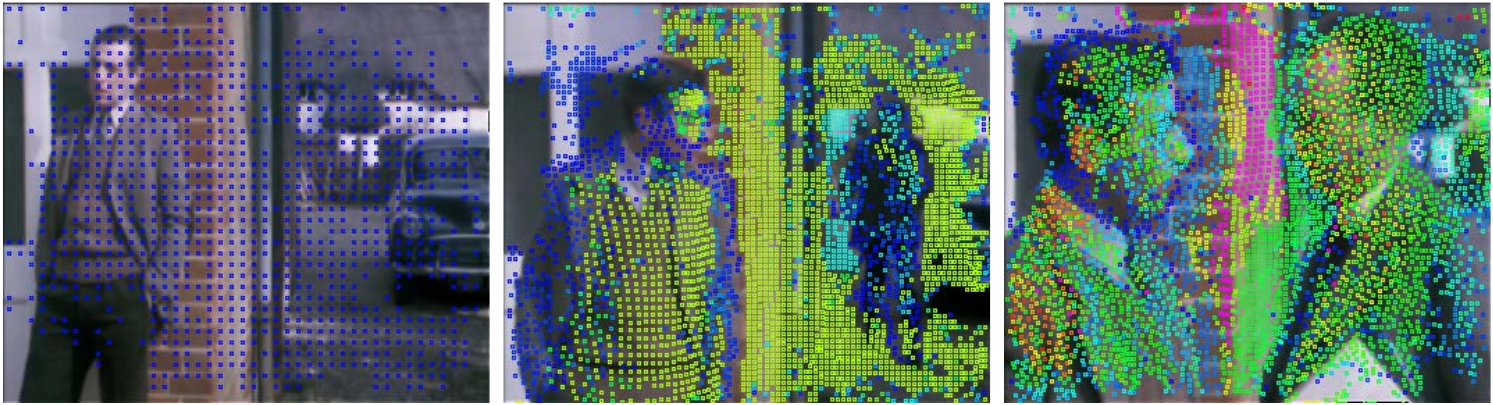
\includegraphics[width=7.0in]{images/trajectories.png}
  \caption{Von links nach rechts: Das erste Frame ursprünglichen Punkt. Sie wurden nur dort initialisiert, wo auch genügend Struktur vorhanden ist.
    Frames 211 und 400 zeigen das Tracking der Punkte. Die Farbe gibt die Dauer des Trackings an (angefangen mit blau als jüngste, über grün, gelb, rot
    und magenta als älteste Punkte).}
  \label{fig:trajectories}
\end{figure*}

Als Grundlage der Trajektorienberechnung dient das von \cite{a001} vorgestellte Verfahren Large Displacement Optical Flow (LDOF).
Dies wird verwendet, um ein optisches Flussfeld $\textbf{w} = (u,v)^T$ zwischen zwei aufeinanderfolgende Bilder einer Videosequenz zu berechnen.

Zunächst wird auf dem ersten Frame des Videos eine Menge von Punkten initialisiert, deren Bewegung auf den darauf folgenden Frames verfolgt werden soll (Abbildung~\ref{fig:trajectories}).
Theoretisch könnte man jedes einzelne Pixel eines Bildes versuchen zu verfolgen, jedoch würde dies zu einem ungemeinen Anstieg der erforderlichen
Rechenkraft führen, zum anderen sind besonders Punkte, die in Bereichen ohne Struktur liegen nur sehr schwer zu verfolgen. Daher werden die Punkte entfernt,
die keine Struktur besitzen, bzw. deren zweiter Eigenwert $\lambda_2$ des Strukturtensors
\begin{equation}
  J_\rho = K_\rho \sum \limits_{k=1}^3 (\nabla I_k)(\nabla I_k)^T
\end{equation}
einen verhältnissmäßig kleinen Wert annimmt. Dabei entspricht $K_p$ einem Gauß-Filter mit Standardabweichung $\rho = 1$ und
$\nabla I_k$ dem Gradient im Farbkanal $k$.

Jeder dieser Punkte kann nun über den zuvor bestimmten optischen Fluss auf das nächste Frame
\begin{equation}
  (x_{t+1}, y_{t+1})^T = (x_t,y_t)^T + (u_t(x_t,y_t), v_t(x_t,y_t))^T
\end{equation}
verfolgt werden. Da der optische Fluss Subpixel-genau arbeitet, ergeben sich für $x$ und $y$ üblicherweise Koordinatenwerte zwischen dem Gitter.
Eine bilinear Interpolation liefert wieder die entsprechenden Punkte auf dem Gitter.

Um die Richtigkeit der Trajektorien zu gewährleisten, muss zuverlässig erkannt werden, wann ein Punkt verdeckt wird und nicht mehr weiter verfolgt werden
kann. Ansonsten würde ein Punkt die Bewegung von zwei unterschiedlichen Objekten beschreiben. Um einen Punkt auf Okklusion zu testen, wird dazu
der Vorwärts- und Rückwärtsfluss überprüft. Diese sollten im nicht verdeckten Fall genau entgegen gerichtet sein:
$ u_t(x_t,y_t) = -\hat{u}_t(x_t + u_t, y_t + v_t) $ und $ v_t(x_t,y_t) = -\hat{v}_t(x_t + u_t, y_t + v_t) $, wobei
$\hat{\textbf{w}}_t := (\hat{u}_t,\hat{v}_t)^T$ dem optischen Fluss von Frame $t+1$ nach $t$ entspricht. Falls diese Bedingung nicht erfüllt sein sollte,
dann wurde der Punkt in $t+1$ entweder verdeckt oder der Fluss wurde nicht richtig bestimmt. Da es jedoch immer zu kleinen Berechnungsfehlern
im optischen Fluss kommen kann, wird für die Überprüfung eine kleine Toleranz zugelassen, die sich linear zur Bewegungsgeschwindigkeit verhält:
\begin{equation}
  | \textbf{w} + \hat{\textbf{w}}|^2 < 0.01 (|\textbf{w}|^2 + |\hat{\textbf{w}}|^2) + 0.5
\end{equation}

Des weiteren werden Punkte an Bewegungskanten nicht weiter verfolgt, da die genaue Schätzung der Grenzen durch den optischen Fluss immer leicht
variiert. Dies kann zu einem ähnlichen Effekt wie bei der Okklusion führen, bei dem ein Punkt plötzlich auf die andere Seite der Grenze fällt
und somit die Bewegung von zwei unterschiedlichen Objekten beschreibt. Um dies zu verhindern, wird ein zusätzliche Bedingung für die korrekte
Verfolgung eingeführt:
\begin{equation}
  |\nabla u|^2 + |\nabla v|^2 > 0.01 |\textbf{w}|^2 + 0.002
\end{equation}

Letztendlich wird noch versucht, die leeren Bereiche des Bildes, die durch Okklusion enstanden sind, wieder zu füllen. Daher werden in jedem neuen Frame
neue Punkte auf die gleiche Weise wie im ersten Bild initialisiert.


\subsection{Segmentierung von Punkttrajektorien}

\begin{figure*}[bt]\centering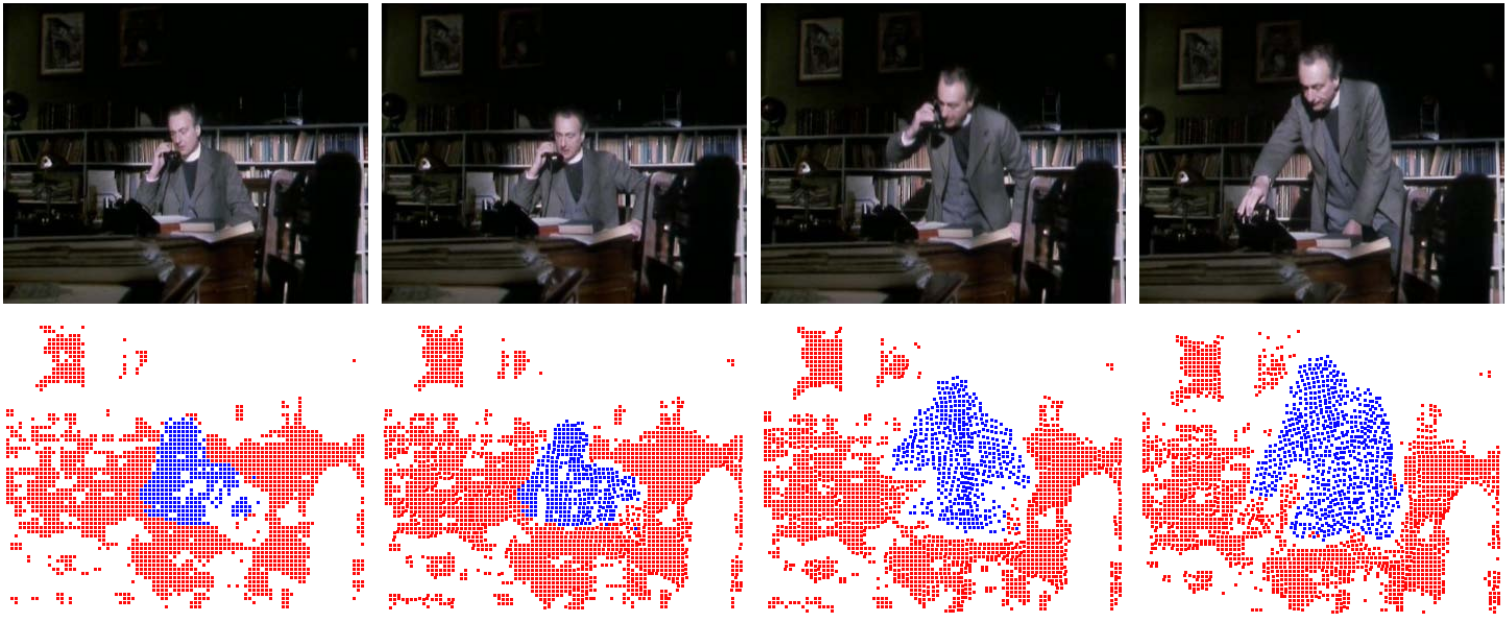
\includegraphics[width=7.0in]{images/motion.png}
  \caption{Frames 0, 30, 50, 80 eines Teils aus dem Film \emph{Miss Marple: Murder at the vicarage}. Bis zu Frame 30 gibt es kaum Bewegung,
  da die Person sitzt. Die meiste Information wird geliefert, sobald sie aufsteht. Mit Hilfe der Langezeit-Verfolgung, ist diese Information
auch im erste Frame verfügbar.}
  \label{fig:motion}
\end{figure*}


Nachdem nun die Punkttrajektorien zur Verfügung stehen, wird das Objektsegmentierungsverfahren von \cite{a001} zum Clustern verwendet.
Wie in Abbildung~\ref{fig:trajectories} zu sehen ist, können diese Trajektorien sich über sehr lange Zeiträume erstrecken, können zeitweise
verdeckt werden oder zu jeder Zeit neue dazukommen. Würden nun nur die Trajektorien ausgewählt werden, die die gesamte Videosequenz abdecken,
würde das Set am Ende sehr klein oder sogar ganz leer sein. Daher wird zum Vergleich eine paarweise Affinität zwischen allen Trajektorien definiert,
die mindestens ein gemeinsames Frame besitzen. Diese Affinitäten definieren dann einen Graphen, auf dem anschließend ein Spectral Clustering Verfahren
angewendet werden kann. Durch diese Transitivität können selbst Trajektorien, die niemals ein gemeinsames Frame besitzen,
dem selben Cluster zugeordnet werden.

Schließlich gilt es noch zu beachten, dass es zu Situationen kommen kann, in denen man zwei Objekte mit gleicher Bewegung nicht von einander unterscheiden
kann. Die tatsächliche Information liegt daher nicht in der gemeinsamen Bewegung, sonderen im Bewegungsunterschied. Sobald also zum Beispiel eine Person
ihre Bewegungsrichtung ändert und diese sich nicht mehr mit der anderen Person gleicht, besitzt man eine genug Daten, um zu wissen, dass diese beiden
Regionen im Bild nicht zusammen gehören (Abbildung~\ref{fig:motion}).

Daraus kann nun eine Distanzmetrik zwischen zwei Trajektorien $A$ und $B$ definierte werden
\begin{equation}
  d^2(A,B) = \mathrm{max}_t d_t^2(A,B),
\end{equation}
an der Stelle, an der der Bewegungsunterschied zwischen zwei Punkten am größten ist. Die Distanz zwischen zwei Punkten zum Zeitpunkt $t$ ist definert als:
\begin{equation}
  d_t^2(A,B) = d_{sp}(A,B) \frac{(u_t^A - u_tt^B)^2 + (v_t^A - v_t^B)^2}{5\sigma_t^2}
\end{equation}
Dabei bezeichneit $d_{sp}(A,B)$ die mittlere, euklidische Distanz von A und B in einem gemeinsame Zeitfenster. Diese räumliche Gewichtung weist
nahen Punkten eine größere Bedeutung zu. $u_t := x_{t+5} - x_t$ und $v_t := y_{t+5} - y_t$ bezeichnet die gemittelte Bewegung eines Punktes über fünf Frames,
was zusätzliche Genauigkeit bietet. $\sigma_t$ schließlich fügt eine Normalisierung der Distanz hinzu
\begin{equation}
  \sigma_t = min_{a\in\{A,B\}} \sum \limits_{t'=1}^5 \sigma(x_{t+t'}^a,y_{t+t'}^a,t+t'),
\end{equation}
wobei $\sigma : \mathbb{R}^3 \rightarrow \mathbb{R}$ die Varianz des lokalen optischen Flusses darstellt. Diese Normalisierung soll sicherstellen, dass
schnelle und langsame Bewegungen gleichermaßen behandelt werden.

Schließlich werden diese Distanzen mittels
\begin{equation}
  w(A,B)= \mathrm{exp}(-\lambda d^2(A,B)), \quad \lambda = 0.1
\end{equation}
in Affinitäten umgewandelt, die dann eine $n \times n$ Matrix $W$ für die gesamte Sequenz bilden, wobei $n$ die Anzahl der Trajektorien ist.

Auf diese Affinitätsmatrix können nun gewöhnliche Clusterverfahren angewendet werden. Die Authoren von \cite{007} stellen jedoch auch
eine anpasste Variante des Spectral Clusterings vor, dass um einen räumlichen Regularisierer erweitert wurde, mit dem Ziel, Übersegmentierungen zu vermeiden.


%%% Local Variables: 
%%% mode: latex
%%% TeX-master: "../main"
%%% End: 

\section{Rendering}

Lorem ipsum dolor sit amet, consetetur sadipscing elitr, sed diam
nonumy eirmod tempor invidunt ut labore et dolore magna aliquyam erat,
sed diam voluptua. At vero eos et accusam et justo duo dolores et ea
rebum. Stet clita kasd gubergren, no sea takimata sanctus est Lorem
ipsum dolor sit amet. Lorem ipsum dolor sit amet, consetetur
sadipscing elitr, sed diam nonumy eirmod tempor invidunt ut labore et
dolore magna aliquyam erat, sed diam
voluptua~\cite{kitware2003,Max:1995:OMF}. At vero eos et accusam et
justo duo dolores et ea rebum. Stet clita kasd gubergren, no sea
takimata sanctus est Lorem ipsum dolor sit amet. Lorem ipsum dolor sit
amet, consetetur sadipscing elitr, sed diam nonumy eirmod tempor
invidunt ut labore et dolore magna aliquyam erat, sed diam
voluptua. At vero eos et accusam et justo duo dolores et ea
rebum. Stet clita kasd gubergren, no sea takimata sanctus est Lorem
ipsum dolor sit amet.

Duis autem vel eum iriure dolor in hendrerit in vulputate velit esse
molestie consequat, vel illum dolore eu feugiat nulla facilisis at
vero eros et accumsan et iusto odio dignissim qui blandit praesent
luptatum zzril delenit augue duis dolore te feugait nulla
facilisi~\cite{notes2002}. Lorem ipsum dolor sit amet, consectetuer
adipiscing elit, sed diam nonummy nibh euismod tincidunt ut laoreet
dolore magna aliquam erat volutpat.

Ut wisi enim ad minim veniam, quis nostrud exerci tation ullamcorper
suscipit lobortis nisl ut aliquip ex ea commodo consequat. Duis autem
vel eum iriure dolor in hendrerit in vulputate velit esse molestie
consequat, vel illum dolore eu feugiat nulla facilisis at vero eros et
accumsan et iusto odio dignissim qui blandit praesent luptatum zzril
delenit augue duis dolore te feugait nulla facilisi.

\section{Exposition}

Lorem ipsum dolor sit amet, consetetur sadipscing elitr, sed diam
nonumy eirmod tempor invidunt ut labore et dolore magna aliquyam erat,
sed diam voluptua. At vero eos et accusam et justo duo dolores et ea
rebum. Stet clita kasd gubergren, no sea takimata sanctus est Lorem
ipsum dolor sit amet. Lorem ipsum dolor sit amet, consetetur
sadipscing elitr, sed diam nonumy eirmod tempor invidunt ut labore et
dolore magna aliquyam erat, sed diam voluptua. At vero eos et accusam
et justo duo dolores et ea rebum. Stet clita kasd gubergren, no sea
takimata sanctus est Lorem ipsum dolor sit amet. Lorem ipsum dolor sit
amet, consetetur sadipscing elitr, sed diam nonumy eirmod tempor
invidunt ut labore et dolore magna aliquyam erat, sed diam
voluptua. At vero eos et accusam et justo duo dolores et ea
rebum~\cite{ware:2004:IVP}. Stet clita kasd gubergren, no sea takimata
sanctus est Lorem ipsum dolor sit amet.

Duis autem vel eum iriure dolor in hendrerit in vulputate velit esse
molestie consequat, vel illum dolore eu feugiat nulla facilisis at
vero eros et accumsan et iusto odio dignissim qui blandit praesent
luptatum zzril delenit augue duis dolore te feugait nulla
facilisi. Lorem ipsum dolor sit amet, consectetuer adipiscing elit,
sed diam nonummy nibh euismod tincidunt ut laoreet dolore magna
aliquam erat volutpat~\cite{kindlmann:1999:SAG}.

Ut wisi enim ad minim veniam, quis nostrud exerci tation ullamcorper
suscipit lobortis nisl ut aliquip ex ea commodo
consequat~\cite{levoy:1989:DSV}. Duis autem vel eum iriure dolor in
hendrerit in vulputate velit esse molestie consequat, vel illum dolore
eu feugiat nulla facilisis at vero eros et accumsan et iusto odio
dignissim qui blandit praesent luptatum zzril delenit augue duis
dolore te feugait nulla facilisi.

Lorem ipsum dolor sit amet, consetetur sadipscing elitr, sed diam
nonumy eirmod tempor invidunt ut labore et dolore magna aliquyam erat,
sed diam voluptua. At vero eos et accusam et justo duo dolores et ea
rebum. Stet clita kasd gubergren, no sea takimata sanctus est Lorem
ipsum dolor sit amet. Lorem ipsum dolor sit amet, consetetur
sadipscing elitr, sed diam nonumy eirmod tempor invidunt ut labore et
dolore magna aliquyam erat, sed diam voluptua. At vero eos et accusam
et justo duo dolores et ea rebum. Stet clita kasd gubergren, no sea
takimata sanctus est Lorem ipsum dolor sit amet. Lorem ipsum dolor sit
amet, consetetur sadipscing elitr, sed diam nonumy eirmod tempor
invidunt ut labore et dolore magna aliquyam erat, sed diam
voluptua. At vero eos et accusam et justo duo dolores et ea
rebum. Stet clita kasd gubergren, no sea takimata sanctus est Lorem
ipsum dolor sit amet.

Lorem ipsum dolor sit amet, consetetur sadipscing elitr, sed diam
nonumy eirmod tempor invidunt ut labore et dolore magna aliquyam erat,
sed diam voluptua. At vero eos et accusam et justo duo dolores et ea
rebum. Stet clita kasd gubergren, no sea takimata sanctus est Lorem
ipsum dolor sit amet. Lorem ipsum dolor sit amet, consetetur
sadipscing elitr, sed diam nonumy eirmod tempor invidunt ut labore et
dolore magna aliquyam erat, sed diam voluptua. At vero eos et accusam
et justo duo dolores et ea rebum. Stet clita kasd gubergren, no sea
takimata sanctus est Lorem ipsum dolor sit amet. Lorem ipsum dolor sit
amet, consetetur sadipscing elitr, sed diam nonumy eirmod tempor
invidunt ut labore et dolore magna aliquyam erat, sed diam
voluptua. At vero eos et accusam et justo duo dolores et ea
rebum. Stet clita kasd gubergren, no sea takimata sanctus est Lorem
ipsum dolor sit amet.

Lorem ipsum dolor sit amet, consetetur sadipscing elitr, sed diam
nonumy eirmod tempor invidunt ut labore et dolore magna aliquyam erat,
sed diam voluptua. At vero eos et accusam et justo duo dolores et ea
rebum. Stet clita kasd gubergren, no sea takimata sanctus est Lorem
ipsum dolor sit amet. Lorem ipsum dolor sit amet, consetetur
sadipscing elitr, sed diam nonumy eirmod tempor invidunt ut labore et
dolore magna aliquyam erat, sed diam voluptua.


\begin{figure}[tb]
  \centering
  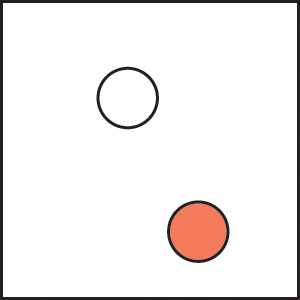
\includegraphics[width=1.5in]{sample}
  \caption{\label{fig:sample} Beispielillustration.}
\end{figure}

\begin{equation}
  \sum_{j=1}^{z} j = \frac{z(z+1)}{2}
\end{equation}

Lorem ipsum dolor sit amet, consetetur sadipscing elitr, sed diam
nonumy eirmod tempor invidunt ut labore et dolore magna aliquyam erat,
sed diam voluptua. At vero eos et accusam et justo duo dolores et ea
rebum. Stet clita kasd gubergren, no sea takimata sanctus est Lorem
ipsum dolor sit amet. Lorem ipsum dolor sit amet, consetetur
sadipscing elitr, sed diam nonumy eirmod tempor invidunt ut labore et
dolore magna aliquyam erat, sed diam voluptua. At vero eos et accusam
et justo duo dolores et ea rebum. Stet clita kasd gubergren, no sea
takimata sanctus est Lorem ipsum dolor sit amet. Lorem ipsum dolor sit
amet, consetetur sadipscing elitr, sed diam nonumy eirmod tempor
invidunt ut labore et dolore magna aliquyam erat, sed diam
voluptua. At vero eos et accusam et justo duo dolores et ea
rebum. Stet clita kasd gubergren, no sea takimata sanctus est Lorem
ipsum dolor sit amet.

Lorem ipsum dolor sit amet, consetetur sadipscing elitr, sed diam
nonumy eirmod tempor invidunt ut labore et dolore magna aliquyam erat,
sed diam voluptua. At vero eos et accusam et justo duo dolores et ea
rebum. Stet clita kasd gubergren, no sea takimata sanctus est Lorem
ipsum dolor sit amet. Lorem ipsum dolor sit amet, consetetur
sadipscing elitr, sed diam nonumy eirmod tempor invidunt ut labore et
dolore magna aliquyam erat, sed diam voluptua. At vero eos et accusam
et justo duo dolores et ea rebum. Stet clita kasd gubergren, no sea
takimata sanctus est Lorem ipsum dolor sit amet. Lorem ipsum dolor sit
amet, consetetur sadipscing elitr, sed diam nonumy eirmod tempor
invidunt ut labore et dolore magna aliquyam erat, sed diam
voluptua. At vero eos et accusam et justo duo dolores et ea
rebum. Stet clita kasd gubergren, no sea takimata sanctus est Lorem
ipsum dolor sit amet.

\begin{table}
  %% Table captions on top in journal version
  \caption{\label{tab:vis_accept} Vis Paper Acceptance Rate}
  \scriptsize
  \begin{center}
    \begin{tabular}{cccc}
      Year & Submitted & Accepted & Accepted (\%)\\
      \hline
      1994 &  91 & 41 & 45.1\\
      1995 & 102 & 41 & 40.2\\
      1996 & 101 & 43 & 42.6\\
      1997 & 117 & 44 & 37.6\\
      1998 & 118 & 50 & 42.4\\
      1999 & 129 & 47 & 36.4\\
      2000 & 151 & 52 & 34.4\\
      2001 & 152 & 51 & 33.6\\
      2002 & 172 & 58 & 33.7\\
      2003 & 192 & 63 & 32.8\\
      2004 & 167 & 46 & 27.6\\
      2005 & 268 & 88 & 32.8\\
      2006 & 228 & 63 & 27.6
    \end{tabular}
  \end{center}
\end{table}


Lorem ipsum dolor sit amet, consetetur sadipscing elitr, sed diam
nonumy eirmod tempor invidunt ut labore et dolore magna aliquyam erat,
sed diam voluptua. At vero eos et accusam et justo duo dolores et ea
rebum. Stet clita kasd gubergren, no sea takimata sanctus est Lorem
ipsum dolor sit amet. Lorem ipsum dolor sit amet, consetetur
sadipscing elitr, sed diam nonumy eirmod tempor invidunt ut labore et
dolore magna aliquyam erat, sed diam voluptua. At vero eos et accusam
et justo duo dolores et ea rebum. Stet clita kasd gubergren, no sea
takimata sanctus est Lorem ipsum dolor sit amet.

\begin{figure*}[tb]
  \centering
  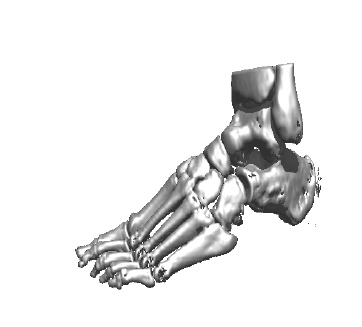
\includegraphics[width=4cm]{images/foot1}\hfill
  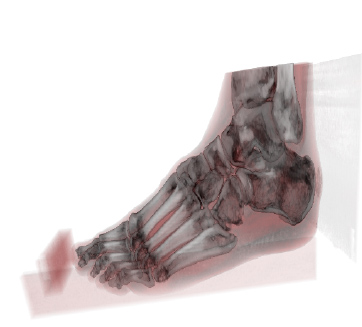
\includegraphics[width=4cm]{images/foot2}\hfill
  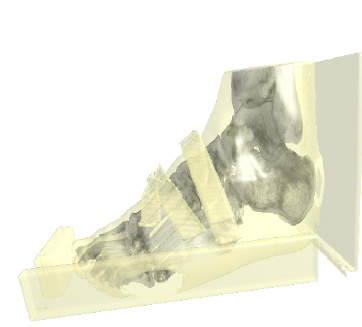
\includegraphics[width=4cm]{images/foot3}\hfill
  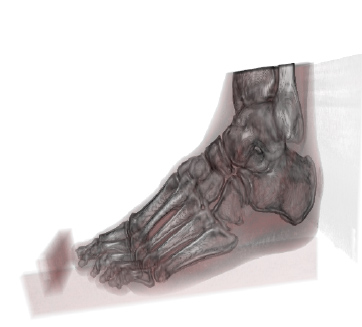
\includegraphics[width=4cm]{images/foot4}
  \caption{Illustration "uber beide Textspalten hinweg. Auch
    Illustrationen m"ussen entsprechend den Quellen gekennzeichnet
    werden. \cite{strengert2006spectral}}
  \label{fig:multicolumn}
\end{figure*}


Lorem ipsum dolor sit amet, consetetur sadipscing elitr, sed diam
nonumy eirmod tempor invidunt ut labore et dolore magna aliquyam erat,
sed diam voluptua. At vero eos et accusam et justo duo dolores et ea
rebum. Stet clita kasd gubergren, no sea takimata sanctus est Lorem
ipsum dolor sit amet. Lorem ipsum dolor sit amet, consetetur
sadipscing elitr, sed diam nonumy eirmod tempor invidunt ut labore et
dolore magna aliquyam erat, sed diam voluptua. At vero eos et accusam
et justo duo dolores et ea rebum. Stet clita kasd gubergren, no sea
takimata sanctus est Lorem ipsum dolor sit amet. Lorem ipsum dolor sit
amet, consetetur sadipscing elitr, sed diam nonumy eirmod tempor
invidunt ut labore et dolore magna aliquyam erat, sed diam
voluptua. At vero eos et accusam et justo duo dolores et ea
rebum. Stet clita kasd gubergren, no sea takimata sanctus est Lorem
ipsum dolor sit amet.


\subsection{Mezcal Head}

Duis autem~\cite{Lorensen:1987:MCA} vel eum iriure dolor in hendrerit
in vulputate velit esse molestie consequat, vel illum dolore eu
feugiat nulla facilisis at vero eros et accumsan et iusto odio
dignissim qui blandit praesent luptatum zzril delenit augue duis
dolore te feugait nulla facilisi. Lorem ipsum dolor sit amet,
consectetuer adipiscing elit, sed diam nonummy nibh euismod tincidunt
ut laoreet dolore magna aliquam erat volutpat%
\footnote{Fu"snoten erscheinen an der Unterkante der Spalte. Sie
  sollten jedoch vermieden werden, da der Lesefluss gest"ort wird.}.


\subsubsection{Ejector Seat Reservation}

Ut wisi enim ad minim veniam, quis nostrud exerci tation ullamcorper
suscipit lobortis nisl ut aliquip ex ea commodo
consequat~\cite{Nielson:1991:TAD}. Duis autem vel eum iriure dolor in
hendrerit in vulputate velit esse molestie consequat, vel illum dolore
eu feugiat nulla facilisis at vero eros et accumsan et iusto odio
dignissim qui blandit praesent luptatum zzril delenit augue duis
dolore te feugait nulla facilisi.

\paragraph{Rejected Ejector Seat Reservation}

Ut wisi enim ad minim veniam, quis nostrud exerci tation ullamcorper
suscipit lobortis nisl ut aliquip ex ea commodo consequat. Duis autem
vel eum iriure dolor in hendrerit in vulputate velit esse molestie

\section{Zusammenfassung}

Die Arbeit von P. Ochs und T. Brox stellt ein variationales, hierarchisches Model vor, um aus dünnen, unvollständingen Sets von Labeln dichte Segmente
zu generieren. Der variationale Ansatz optimiert dabei gleichzeit kontinuerliche Funktionen auf mehreren Superpixelebenen, und ist, nach Aussagen
der Authoren, der erste variationale Ansatz, der auf mehreren Ebenen arbeitet. Bei verschiedenen Experimenten stellten die Authoren fest,
dass ihre Segmentierung sogar noch die Genauigkeit der unvollständingen Eingabesets verbessert. Ziel der Arbeit war es, die
Forschung in Richtung der unbeaufsichtigten Objektsegmentierung und somit letztendich auch dem vollständig unbeaufsichtigten Lernens voranzubringen.

%%% Local Variables: 
%%% mode: latex
%%% TeX-master: "../main"
%%% End: 


\bibliographystyle{abbrv}
%% use following if all content of bibtex file should be shown
% \nocite{*}
\bibliography{literatur}
\end{document}
